%%%%%%%%%%%%%%%%%%%%%%%%%%%%%%%%%%%%%%%%%%%%%%%%%%%%%%%%%%%%%%%%%%%%%
% In English:
%    This is a Latex template for São Paulo Research Foudation (FAPESP)
%         reports (annual or final).
%    This is the modified version of the original Latex template from
%         following website.
%    Original Source: http://www.howtotex.com
%    For information about FAPESP, check http://www.fapesp.br/en
%    This template targets mainly on reports in Portuguese language.
%    New additions and changes in the latest version:
%        - Added the possibility of including multiple members in the
%          research team, with the commands \memberA{Name of Member A}
%          \memberB{Name of Member B} \memberC{Name of Member C} etc.
%        - Included commands to define project modality and the research
%          agency (if you want to use the same model for other research
%          agencies such as CAPES, CNPq etc).
%
% In Portuguese:
%    Este é um modelo Latex para relatórios (anual ou final) da Fundação
%         de Amparo à pesquisa do Estado de São Paulo (FAPESP).
%    Esta é uma versão modificada do modelo Latex do site supra mencionado.
%    Para informações sobre a FAPESP, verifique http://www.fapesp.br
%    Esse modelo foca principalmente nos relatórios escritos em Português.
%    Novas adições e alterações na última versão:
%       - Foi adicionada a possibilidade de incluir vários membros no
%         grupo de pesquisas, com os comandos \membroA{Nome do Membro A}
%         \membroB{} \membroC{} etc.
%       - Foram incluídos comandos para definir modalidade de projeto e
%         agência de fomento (caso queira utilizar o mesmo modelo para
%         outras agências, CAPES, CNPq etc).
%
% Author/Autor: André Leon Sampaio Gradvohl, Dr.
% Email:        andre.gradvohl@gmail.com
% Lattes CV:    http://lattes.cnpq.br/9343261628675642
% GitHub: http://gradvohl.github.io/
%
% Last update/Última versão: 19/Feb/2018
%
%%%%%%%%%%%%%%%%%%%%%%%%%%%%%%%%%%%%%%%%%%%%%%%%%%%%%%%%%%%%%%%%%%%%%%
\documentclass[12pt]{report}
\usepackage[a4paper]{geometry}
\usepackage[utf8]{inputenc}
\usepackage[english,portuguese]{babel}
\usepackage[myheadings]{fullpage}
\usepackage[T1]{fontenc}
\usepackage{fancyhdr}
\usepackage{setspace}
\usepackage{sectsty}
\usepackage{url}

%%% iniciar capitulo na mesma pagina (Mateus) %%%
\usepackage{etoolbox}
\makeatletter %inicio da modificacao (iniciar capitulo na msma pag)
\patchcmd{\chapter}{\if@openright\cleardoublepage\else\clearpage\fi}{}{}{}
\makeatother %fim da modificacao
%%% iniciar capitulo na mesma pagina (Mateus) %%%

%%------
%% Comandos gerais
%% Observação: o arquivo "comandos.tex" tem que estar presente.
%%------
%%%%%%%%%%%%%%%%%%%%%%%%%%%%%%%%%%%%%%%%%%%%%%%%%%%%%%%%%%%%%%%%%%%%%
% In English:
%    This is a list of commands specification for FAPESP reports.
%
% In Portuguese:
%    Esta é uma lista de especificação de comandos para relatórios
% da Fundação de Amparo à pesquisa do Estado de São Paulo (FAPESP).
%
% Author/Autor: André Leon Sampaio Gradvohl, Dr.
% Email:        andre.gradvohl@gmail.com
% Lattes CV:    http://lattes.cnpq.br/9343261628675642
%
% Last update/Última versão: 11/Sep/2016
%%%%%%%%%%%%%%%%%%%%%%%%%%%%%%%%%%%%%%%%%%%%%%%%%%%%%%%%%%%%%%%%%%%%%%

\newcommand{\HRule}[1]{\rule{\linewidth}{#1}}
\setcounter{tocdepth}{3}
\setcounter{secnumdepth}{3}

\newcommand{\titulo}[1]{\def\meuTitulo{#1}}
\newcommand{\tituloIngles}[1]{\def\meuTituloIngles{#1}}
\newcommand{\numProjeto}[1]{\def\numFAP{#1}}
\newcommand{\tipoRelatorio}[1]{\def\tipoRelat{#1 }} %o espaço depois do #1 é importante
\newcommand{\modalidadeProjeto}[1]{\def\modProjeto{#1}}
\newcommand{\agFomento}[2]{\def\agFom{#1} \def\siglaAgFom{#2}} %extenso Sigla
\newcommand{\autor}[1]{\def\nomeAutor{#1}}
\newcommand{\cidade}[1]{\def\nomeCidade{#1}}
\newcommand{\universidade}[1]{\def\nomeUniversidade{#1}}
\newcommand{\faculdade}[1]{\def\nomeFaculdade{#1}}
\newcommand{\periodoVigencia}[1]{\def\periodVig{#1}}
\newcommand{\periodoRelatorio}[1]{\def\periodRelat{#1}}
\newcommand{\orientador}[1]{\def\nomeOrientador{#1}}

\newcommand\namegroup[2]{%
   \begin{minipage}[t]{0.4\textwidth}
   \hspace{0.6cm}
   \begin{tikzpicture}
   \node[anchor=south east,inner sep = 0](signF){\includegraphics[width=5cm]{#2}};
   \end{tikzpicture}
   \vspace*{0.1cm}  % leave some space above the horizontal line
   \hrule
   \vspace{1mm} % just a bit more whitespace below the line
   \centering
   \begin{tabular}[t]{c}
   #1
   \end{tabular}
   \end{minipage}}

\author{}
\date{}

%Definição de membros da equipe de pesquisas
\newcommand{\membroA}[1]{\def\nomeMembroA{#1}}
\newcommand{\membroB}[1]{\def\nomeMembroB{#1}}
\newcommand{\membroC}[1]{\def\nomeMembroC{#1}}
\newcommand{\membroD}[1]{\def\nomeMembroD{#1}}
\newcommand{\membroE}[1]{\def\nomeMembroE{#1}}
\newcommand{\membroF}[1]{\def\nomeMembroF{#1}}

\newcommand{\Figure}[1]{Figura~\ref{fig:#1}}
\newcommand{\Table}[1] {Tabela~\ref{#1}}
\newcommand{\Equation}[1] {Equa\c{c}\~ao~\ref{#1}}
\newcommand{\addFigure}[3] { %Parametros scale, fig_name, caption
    \begin{figure}[!hbt]
      \centering
      \includegraphics[scale=#1]{figures/}
      \caption{#3}\label{fig:#2}
    \end{figure}
}

\newcommand{\geraTitulo}{
\clearpage
\begin{titlepage}
  \begin{center}
      \vspace*{-3cm}
       { \setstretch{.5}
         \textsc{\nomeUniversidade} \\
         \HRule{.2pt}\\
         \textsc{\nomeFaculdade}
       }

       \vspace{5.5cm}

       \Large \textbf{\textsc{\meuTitulo}}
 	  \HRule{1.5pt} \\ [0.5cm]
       \linespread{1}
       \large Relatório Científico
       \ifdefined\tipoRelat
            \tipoRelat
       \fi
       do projeto
       \ifdefined\modProjeto
           na modalidade \modProjeto,
       \fi
       fomentado pela \agFom. \\
   	   \HRule{1.5pt} \\ [0.5cm]

       \ifdefined\numFAP
          Projeto \siglaAgFom~\texttt{\#\numFAP}
          \\ [0.5cm]
       \fi
        Aluno: \nomeAutor \\
        Orientadora: \nomeOrientador \\[5.cm]

        % aqui começa a adicao das linhas de assinatura
        %Aluno: \tikz\draw [thick,solid] (0,0) -- (6,0); \\[.5cm]
        %Orientador: \tikz\draw [thick,solid] (0,0) -- (5.5,0);


        \namegroup{Aluno}{fig/assinatura-mateus.png}
        \hspace{1.5cm}
        \namegroup{Orientadora}{fig/assinatura-funchal.png}

        %\begin{minipage}[t]{0.4\textwidth}
        %\vspace*{1.5cm}
        %\hrule
        %\vspace{1mm}
        %\centering
        %\begin{tabular}[t]{c}
        %Aluno
        %\end{tabular}
        %\hspace{1.5cm}
        %\begin{minipage}[t]{0.4\textwidth}
        %\vspace*{1.5cm}
        %\hrule
        %\vspace{1mm}
        %\centering
        %\begin{tabular}[t]{c}
        %Aluno
        %\end{tabular}
        %\end{minipage}
        %%\hfill

        \vfill

        {\normalsize  \nomeCidade, \today}
 \end{center}
 \end{titlepage}
}

\usepackage{titlesec}
\titleformat{\chapter}{\normalfont\LARGE\bfseries}{\thechapter}{1em}{}
\titlespacing*{\chapter}{0pt}{3.5ex plus 1ex minus .2ex}{2.3ex plus .2ex}

%----------------------------------------------------------------------
% Cabeçalho e rodapé
%----------------------------------------------------------------------
\pagestyle{fancy}
\fancyhf{} % Limpa todos os campos de header and footer fields
\renewcommand{\headrulewidth}{0pt}
\fancyfoot[R]{\thepage}

\addto\captionsportuguese{\renewcommand{\contentsname}{Sumário}}
\addto\captionsportuguese{\renewcommand{\bibname}{Referências Bibliográficas}}

%------
% Resumo e Abstract
%------
\newcommand{\Resumo}[1]{
   \begin{otherlanguage}{portuguese}
       \addcontentsline{toc}{chapter}{Resumo}
       \begin{abstract} \thispagestyle{plain} \setcounter{page}{2}
          #1
        \end{abstract}
   \end{otherlanguage}
} %end \Resumo

\newcommand{\Abstract}[1]{
   \begin{otherlanguage}{english}
      \addcontentsline{toc}{chapter}{Abstract}
      \begin{abstract} \thispagestyle{plain} \setcounter{page}{3}
       #1
      \end{abstract}
    \end{otherlanguage}
} %end \abstract

%------
% Folha de rosto
%------
\newcommand{\folhaDeRosto}{
   \chapter*{Informações Gerais do Projeto}
   \addcontentsline{toc}{chapter}{Informações Gerais do Projeto}
   \begin{itemize}
      \item Título do projeto:
            \begin{itemize}\item[] \textbf{\meuTitulo} \end{itemize}
      \item Nome do pesquisador responsável:
            \begin{itemize}\item[]\textbf{Profa. \nomeOrientador}\end{itemize}
      \item Instituição sede do projeto:
            \begin{itemize}
               \item[]\textbf{\nomeFaculdade \ da \nomeUniversidade}
            \end{itemize}
      \item Equipe de pesquisa:
            \begin{itemize}
               \ifdefined\nomeMembroA
                 \item[]\textbf{\nomeMembroA}
               \else
                 \item[]\textbf{\nomeAutor}
               \fi
               \ifx\nomeMembroB\undefined\else \item[]\textbf{\nomeMembroB}\fi
               \ifx\nomeMembroC\undefined\else \item[]\textbf{\nomeMembroC}\fi
               \ifx\nomeMembroD\undefined\else \item[]\textbf{\nomeMembroD}\fi
               \ifx\nomeMembroE\undefined\else \item[]\textbf{\nomeMembroE}\fi
               \ifx\nomeMembroF\undefined\else \item[]\textbf{\nomeMembroF}\fi
             \end{itemize}

          \ifdefined \numFAP
             \item Número do projeto de pesquisa:
             \begin{itemize}
                 \item[]\textbf{\numFAP}
             \end{itemize}
          \fi
       \item Período de vigência:
            \begin{itemize}
               \item[]\textbf{\periodVig}
            \end{itemize}
       \item Período coberto por este relatório científico:
            \begin{itemize}
               \item[]\textbf{\periodRelat}
            \end{itemize}
   \end{itemize}
   \clearpage
}

\usepackage{mathtools}
%\usepackage{amsthm}
\usepackage{amsmath}
%\usepackage{nccmath}
\usepackage{amssymb}
%\usepackage{amsfonts}
\usepackage{physics}
%\usepackage{dsfont}
%\usepackage{mathrsfs}
%\usepackage{slashed}    % Feynman slash notation, requires LuaLaTeX
%\usepackage[compat=1.1.0]{tikz-feynman}   % Feynman diagrams

%\usepackage{titling}
\usepackage{indentfirst}
%\usepackage[titletoc,title]{appendix}
%\renewcommand\appendixname{Apêndice}

\usepackage{bm}
%\usepackage{xcolor}
%\usepackage[dvipsnames]{xcolor}
\usepackage{cancel}

%\usepackage{xurl}
\usepackage{hyperref}
\usepackage{cite}

\usepackage{float}
\usepackage{graphicx}
\usepackage{tikz}
\usepackage{caption}
\usepackage{subcaption}

%%%%%%%%%%%%%%%%%%%%%%%%%%%%%%%%%%%%%%%%%%%%%%%%%%%

\newcommand{\eps}{\epsilon}
\newcommand{\vphi}{\varphi}
\newcommand{\cte}{\text{cte}}

\newcommand{\N}{\mathbb{N}}
\newcommand{\Z}{\mathbb{Z}}
\newcommand{\Q}{\mathbb{Q}}
\newcommand{\R}{\mathbb{R}}
\newcommand{\C}{\mathbb{C}}
\renewcommand{\P}{\mathbb{P}}
\renewcommand{\H}{\s{H}}

\newcommand{\0}{\vb{0}}
\newcommand{\1}{\mathds{1}}
\newcommand{\E}{\vb{E}}
\newcommand{\B}{\vb{B}}
\renewcommand{\v}{\vb{v}}
\renewcommand{\r}{\vb{r}}
\newcommand{\p}{\vb{p}}
\newcommand{\q}{\vb{q}}
\newcommand{\F}{\vb{F}}
\newcommand{\dtcp}{\delta_{\text{CP}}}

\newcommand{\s}[1]{\mathcal{#1}}
\renewcommand{\sl}[1]{\slashed{#1}}
\newcommand{\prodint}[2]{\left\langle #1 , #2 \right\rangle}
\newcommand{\cc}[1]{\overline{#1}}
\newcommand{\Eval}[3]{\eval{\left( #1 \right)}_{#2}^{#3}}

\newcommand{\unit}[1]{\; \mathrm{#1}}

\newcommand{\n}{\medskip}
\newcommand{\e}{\quad \mathrm{e} \quad}
\newcommand{\ou}{\quad \mathrm{ou} \quad}
\newcommand{\virg}{\, , \;}
\newcommand{\ptodo}{\forall \,}
\newcommand{\existe}{\exists \,}
\renewcommand{\implies}{\; \Rightarrow \;}
%\newcommand{\eqname}[1]{\tag*{#1}} % Tag equation with name

% MACROS
\newcommand{\dcp}{\delta_{\text{CP}}}

%
%%-----
%% Página de título
%% Observação: As definições que aparecem a seguir comporão a
%%             página de título e a folha de rosto.
%%-----
%% Define o nome da universidade onde o projeto foi desenvolvido.
\universidade{Universidade de São Paulo}
%
%% Define o nome da faculdade onde o projeto foi desenvolvido.
\faculdade{Instituto de Física}
%
%% Define o título do projeto.
\titulo{Física de Neutrinos na Física de Partículas Elementares}
%
%% Define a agencia de Fomento e a abreviatura. O primeiro argumento é o
%% nome por extenso e o segundo a abreviatura.
%% Ambos os argumentos são obrigatórios
\agFomento{Fundação de Amparo à Pesquisa do Estado de São Paulo}{FAPESP}
%
%% Define o tipo de relatório. Pode ser Anual ou Final.
%% Não é obrigatório definir o tipo de relatório.
\tipoRelatorio{Final}
%
%% Define a modalidade de Projeto. Pode ser temático, regular, etc.
\modalidadeProjeto{Iniciação Científica}
%
%% Define o número do projeto.
%% Não é obrigatório definir o número do projeto.
\numProjeto{2021/12401-6}
%
%% Define o autor do relatório.
\autor{Mateus Marques}
\orientador{Dra. Renata Zukanovich Funchal}
%
%% Define a equipe do projeto (incluindo o pesquisador responsável no comando \membroA{}
\membroA{Mateus Marques}
%% Inclua os demais membros do grupo (máximo +5)
\membroB{Renata Zukanovich Funchal}
%\membroC{Francisco}
%\membroD{Joao}
%\membroE{Antonio}
%\membroF{José}
%
%% Define o período da vigência do Projeto.
\periodoVigencia{01/janeiro/2022 a 31/dezembro/2022}
%
%% Define o período coberto pelo relatório.
\periodoRelatorio{11/junho/2022 a 31/dezembro/2022}
%
%% Define a cidade onde o projeto foi desenvolvido.
\cidade{São Paulo}

%%-----
%% Página de título
%% Observação: Os comandos a seguir não devem ser mudados,
%%             exceto caso necessário.
%%-----
\begin{document}
%
%% Define a numeração em romanos.
\pagenumbering{roman}
%
%% Gera a folha de título.
\geraTitulo
%
%% Gera a folha de rosto.
\folhaDeRosto
%
%% Escreva aqui o resumo em português. Fica no Resumo do Projeto Proposto
%\Resumo{
%Neste projeto estamos interessado apenas no valor da bolsa. Não fizemos praticamente
%nada nesse tempo e não pretendemos fazer. Eu apenas pretendo entregar este relatório
%para ficar tudo certo.
%}
%
%% Escreva aqui o resumo em inglês. NAO PRECISA
%\Abstract{
%Same thing but in english.
%}
%
%% Adicionará o sumário.
%% Mantenha o \thispagestyle{empty} e \clearpage
\tableofcontents
\thispagestyle{empty}
\clearpage
%
%% Define a numeração em arábicos.
\pagenumbering{arabic}

%%-----
%% Formatação do título da seção
%%-----
\sectionfont{\scshape}

%%-----
%% Corpo do texto
%%-----
\chapter{Resumo do projeto proposto}\label{chp:resumoProj}

O presente projeto, na área de Física de Partículas Elementares, propõe um estudo teórico e computacional da fenomenologia das oscilações de neutrinos. A investigação desse fenômeno é o principal tópico da fronteira de pesquisa em neutrinos. Como pode ser visto na Seção II.A de \cite{gonzalez}, o Modelo Padrão implica que a massa dos neutrinos é nula. No entanto, a oscilação de sabor leptônico implica, dentre diversas coisas, a existência de autoestados de massa não-nula. Atualmente, essa é uma das mais fortes evidências de que deve haver física além do Modelo Padrão. Neste projeto exploraremos as oscilações de neutrinos em dois contextos.

Primeiramente consideramos os neutrinos trafegando na presença de matéria. Em particular enfatizaremos os neutrinos solares, que possuem imensa relevância histórica devido ao famoso \textit{problema do neutrino solar} (Seção IV.B de \cite{gonzalez}) e que, ainda hoje, mostram-se de grande interesse experimental, havendo associados a eles grandes experimentos mundo à fora, como SuperKamiokande, SNO e Borexino (Seção IV.A de \cite{gonzalez}). Exibiremos nossa simulação numérica e seus resultados, onde utilizamos os parâmetros do grupo NuFIT \cite{nufit} e dados do modelo solar \texttt{BS2005} de J. N. Bahcall \cite{bahcall, bahcall-model}.

Em seguida, no contexto de oscilações no vácuo, apresentaremos nossa simulação numérica do experimento de antineutrinos em reatores nucleares KamLAND \cite{spectral-distortion} para os dados coletados entre 9 de Março, 2002 e 11 de Janeiro, 2004. Realizamos os cálculos das distribuições de eventos para os casos sem oscilação e com oscilação e comparamos nossos resultados com os eventos observados no KamLAND \cite{kamland-data} durante o período considerado.

\pagebreak

\chapter{Realizações do período}\label{chp:realizacoes}

No segundo semestre focamos principalmente na leitura de artigos e na realização de simulações numéricas de neutrinos solares e do experimento KamLAND.

Com relação aos neutrinos solares, estudamos o artigo \cite{efficient-nu} em detalhe com o fim de implementar um algoritmo mais eficiente para calcularmos a evolução do sabor leptônico. Anteriormente utilizávamos um solucionador genérico de equações diferenciais ordinárias (EDOs) para tal propósito. Com esse algoritmo conseguimos calcular a probabilidade de sobrevivência média quando um neutrino deixa o Sol para os diversos tipos de reações que podem produzi-lo.

Quanto ao KamLAND, foram lidos diversos artigos e teses \cite{spectral-distortion, yuber, detwiler, juno, refmodel} com o fim de serem entendidos os ingredientes necessários para fazer a simulação de todos os reatores nucleares relevantes \cite{pris-iaea} e compararmos nossos resultados os dados experimentais \cite{spectral-distortion, kamland-data}.

\section{Oscilações de neutrinos} \label{sec:osc}

A oscilação de neutrinos consiste no fato de que eles interagem apenas em autoestados de sabor $\nu_e, \nu_\mu, \nu_\tau$, associados aos léptons $e^-$, $\mu^-$ e $\tau^-$, mas que evoluem no tempo com uma hamiltoniana que possui outros autoestados, denominados autoestados de massa $\nu_1$, $\nu_2$ e $\nu_3$. Como se observa experimentalmente, as bases $(\nu_e, \nu_\mu, \nu_\tau)$ e $(\nu_1, \nu_2, \nu_3)$ são diferentes. Se por exemplo um neutrino é produzido como $\nu_e$, após sua propagação num certo tempo, existe uma probabilidade de numa interação futura com um detector ele ser observado no estado $\nu_\mu$ ou $\nu_\tau$.


\subsection{Oscilação de dois neutrinos no vácuo} \label{sec:2nu-vacuo}


A relação entre a base de estados de sabor e a de estados de massa é dada por uma transformação unitária $U$ de maneira que
\begin{equation} \label{eq:unitaria}
\ket{\nu_\alpha} = \sum_{j} U_{\alpha j} \ket{\nu_j},
\end{equation}
para $\alpha = e, \mu, \tau$ e $j = 1, 2, 3$. Supondo primeiramente que tenhamos apenas duas gerações de neutrinos, $\nu_e$ e $\nu_\mu$ por exemplo, temos que a matriz $U$ é unitária e $2 \times 2$, podendo assim ser parametrizada por um único ângulo $\theta$
\begin{equation} \label{eq:mix2}
U =
\begin{pmatrix}
\cos\theta & \sin\theta \\
-\sin\theta & \cos\theta
\end{pmatrix}.
\end{equation}

Temos então explicitamente
\begin{equation}
\begin{split}
\ket{\nu_e} &= \cos \theta \ket{\nu_1} + \sin \theta \ket{\nu_2}, \\
\ket{\nu_\mu} &= -\sin \theta \ket{\nu_1} + \cos \theta \ket{\nu_2}.
\end{split}
\end{equation}

As massas associadas aos neutrinos são extremamente pequenas. Isso nos permite considerá-los como partículas que se movem praticamente à velocidade da luz $c = 1$ (utilizando unidades naturais, convencionamos que $c = \hbar = 1$). Fazemos então a seguinte aproximação relativística para a energia $E_i$ de um neutrino no autoestado de massa $\ket{\nu_i}$:
\begin{equation} \label{eq:aprox-energ}
E_i = \sqrt{p^2 + m_i^2} =
p \qty(1 + \frac{m_i^2}{p^2})^{1/2} \approx \; E \qty( 1 + \frac{m_i^2}{2 E^2} ).
\end{equation}

Nos livrando do fator $E$ da equação \ref{eq:aprox-energ} que é comum dentre todos os 3 autoestados de massa (ele gera somente uma fase global), temos que
\begin{equation} \label{eq:mass-eigen}
M \ket{\nu_i} = \frac{m_i^2}{2E} \ket{\nu_i},
\end{equation}
sendo $M$ a matriz hamiltoniana diagonal na base de autoestados de massa. Utilizando agora a transformação unitária \ref{eq:unitaria}, temos que a matriz hamiltoniana $\H$ na base de sabor satisfaz $\H = U M U^\dagger$. Sendo o estado instantâneo $\ket{\nu(t)} = \psi_e(t) \ket{\nu_e} + \psi_\mu(t) \ket{\nu_\mu}$, obtemos pela equação de Schrödinger que
\begin{equation} \label{eq:quase-2nu}
i \, \dv{t}
\begin{pmatrix}
\psi_e \\ \psi_\mu
\end{pmatrix} = \frac{1}{2E}
\begin{pmatrix}
m_1^2 \cos^2\theta + m_2^2 \sin^2 \theta & \Delta m^2 \sin\theta \cos\theta \\
\Delta m^2 \sin\theta \cos\theta & m_1^2 \sin^2\theta + m_2^2 \cos^2\theta
\end{pmatrix}
\begin{pmatrix}
\psi_e \\ \psi_\mu
\end{pmatrix},
\end{equation}
onde $L = ct = t$ é a distância percorrida e o tempo, já que $c = 1$. Novamente, temos um termo global na matriz à direita da equação \ref{eq:quase-2nu} que não contribui para a evolução temporal do sistema. Ao subtraí-lo, a equação se simplifica e vemos que a oscilação depende somente da diferença entre massas ao quadrado $\Delta m^2 = m_2^2 - m_1^2$
\begin{equation} \label{eq:2nu}
i \, \dv{t}
\begin{pmatrix}
\psi_e \\ \psi_\mu
\end{pmatrix} = \frac{\Delta m^2}{4E}
\begin{pmatrix}
-\cos2\theta & \sin2\theta \\
\sin2\theta & \cos2\theta
\end{pmatrix}
\begin{pmatrix}
\psi_e \\ \psi_\mu
\end{pmatrix}.
\end{equation}

A equação \ref{eq:2nu} pode ser resolvida analiticamente sem dificuldades. Partindo da condição inicial $\ket{\nu(0)} = \ket{\nu_e}$ (o neutrino é produzido como $\nu_e$), obtemos que a probabilidade $P(\nu_e \to \nu_e) = 1 - P(\nu_e \to \nu_\mu)$ de que esse neutrino $\nu_e$ sobreviva num tempo $t$ posterior é
\begin{equation} \label{eq:sobrev-2nu}
\boxed{
P(\nu_e \to \nu_e) = \abs{\braket{\nu_e}{\nu(t)}}^2 =
1 - \sin[2](2 \theta) \, \sin[2](\frac{\Delta m^2}{4} \cdot \frac{L}{E}). }
\end{equation}

A equação \ref{eq:sobrev-2nu} vale para unidades naturais. Para utilizarmos $E$ em GeV, $L$ em km e $\Delta m^2$ em eV$^2$, lembre que $1 = c \approx 3 \cdot 10^5 \unit{km/s}$ e $1 = \hbar \approx 6.58 \cdot 10^{-16} \unit{eV \cdot s}$, de maneira que
$$
\frac{\Delta m^2 L}{4E} = \qty(\frac{\Delta m^2}{\text{eV}^2} \frac{L}{\text{km}} \frac{\text{GeV}}{E})
\frac{1}{4} \cdot \frac{\text{eV}^2 \, \text{km}}{10^9 \, \text{eV}} =
\qty(\frac{\Delta m^2}{\text{eV}^2} \frac{L}{\text{km}} \frac{\text{GeV}}{E})
\frac{1}{4 \cdot 10^9 \cdot 3 \cdot 10^5 \cdot 6.58 \cdot 10^{-16}}
$$
\begin{equation}
\frac{\Delta m^2 L}{4E} \approx 1.267 \, \qty(\frac{\Delta m^2}{\text{eV}^2} \frac{L}{\text{km}} \frac{\text{GeV}}{E}).
\end{equation}

Utilizando essas unidades e os parâmetros de outubro de 2021 do NuFIT\footnote{Esses valores foram obtidos para um ajuste de três gerações de neutrinos, incluindo efeitos de matéria, mas vamos usá-los para ilustrar o caso de oscilação em duas gerações no vácuo.} \cite{nufit}, temos que o ângulo $\theta$ de mistura entre $\nu_1$ e $\nu_2$ corresponde a aproximadamente $\theta_{12} = 33.44^\circ$ e que a diferença entre massas ao quadrado $\Delta m^2$ corresponde a $\Delta m_{21}^2 = 7.42 \cdot 10^{-5} \unit{eV^2}$.

Podemos assim observar a oscilação de duas gerações de neutrinos na Figura \ref{fig:2nu-vacuo} em função de $L/E$. Nota-se claramente que, a partir de $L / E$ da ordem de $10000$ (km/GeV), existe uma alta probabilidade $P(\nu_e \to \nu_\mu)$ do nosso neutrino $\nu_e$ inicial ser detectado no sabor $\nu_\mu$.

\begin{figure}[H]
\centering
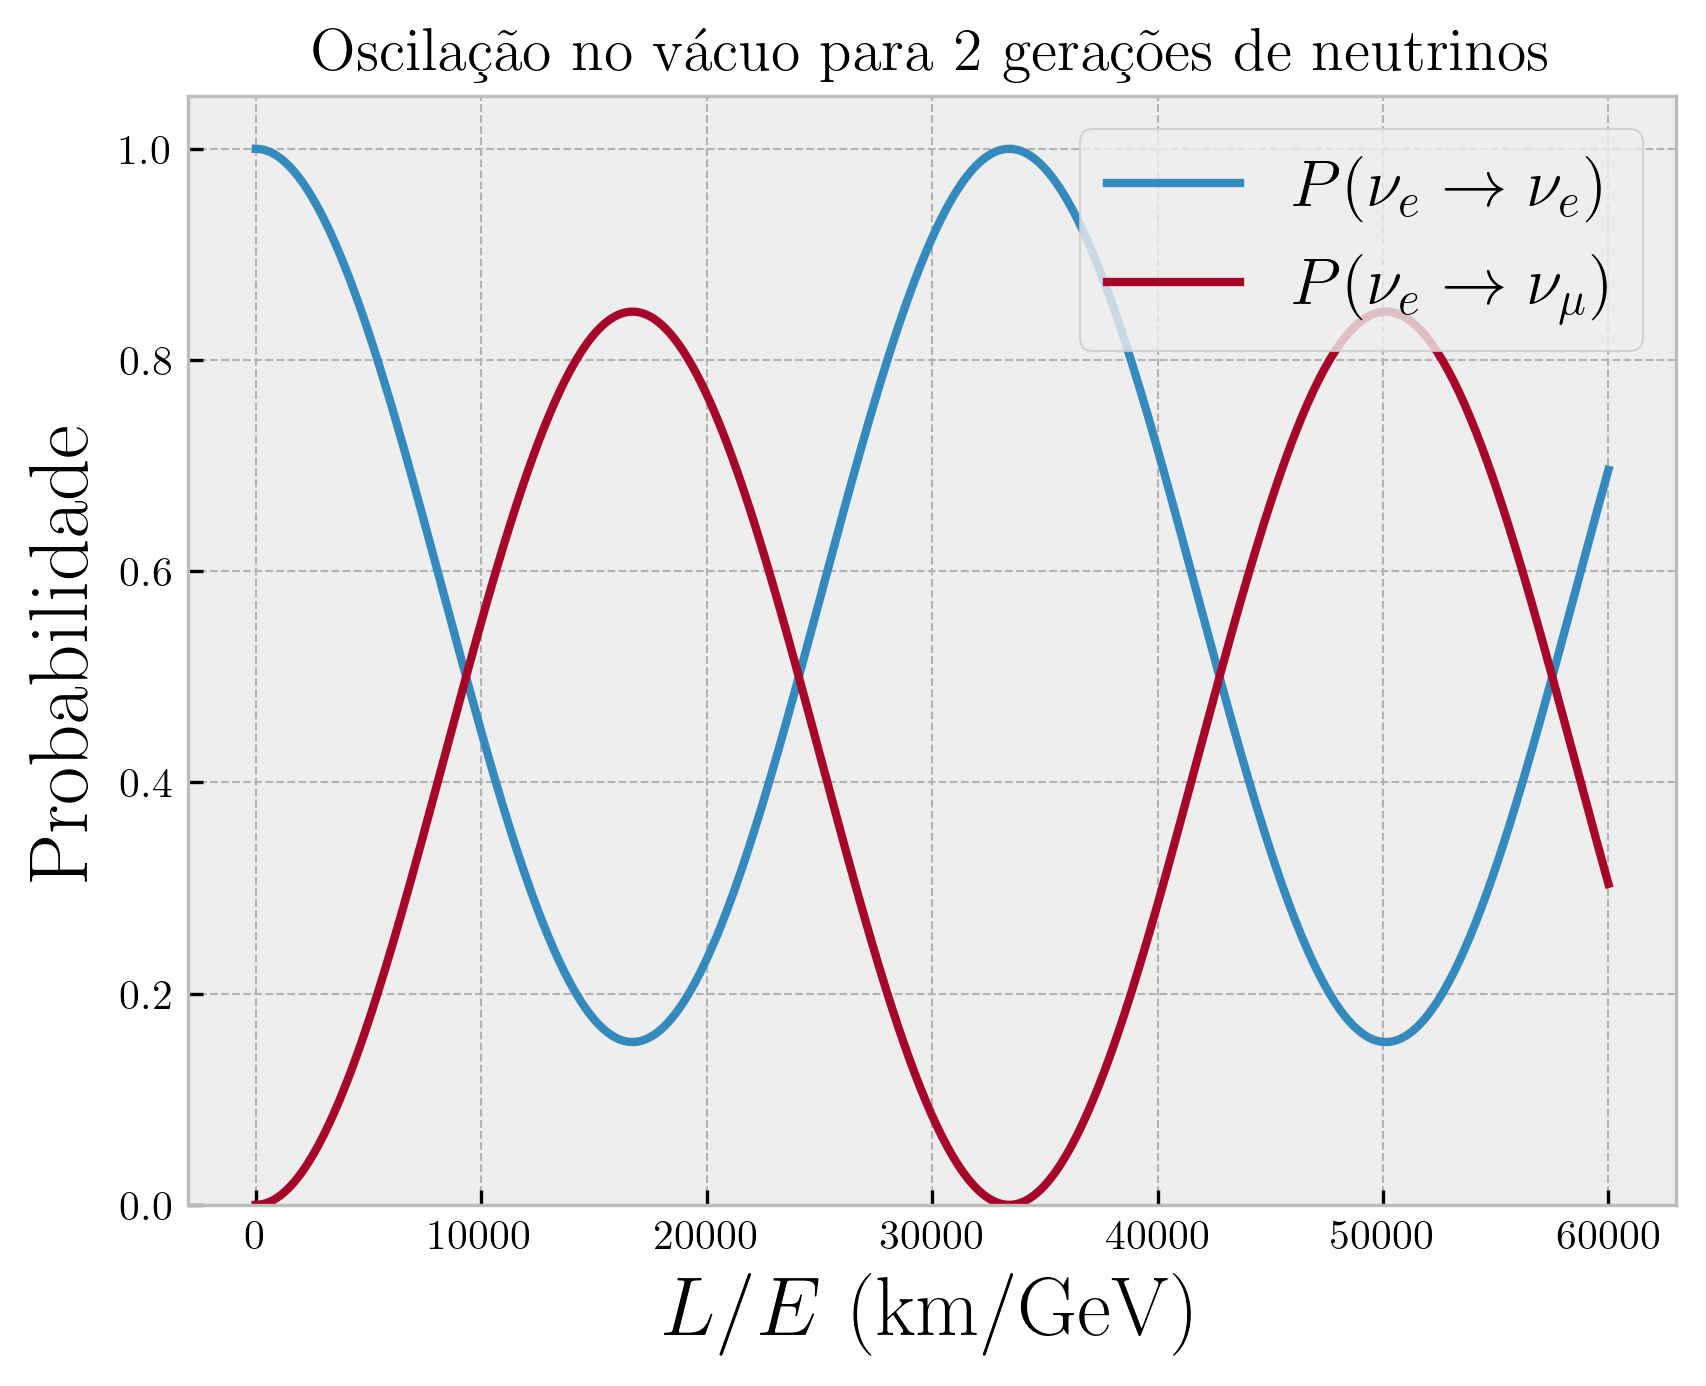
\includegraphics[width=0.52\textwidth]{fig/2nu-vacuo.png}
\caption{Oscilação de sabor no vácuo, com os parâmetros de outubro de 2021 do NuFIT \cite{nufit}, para duas gerações de neutrinos $\nu_e$ e $\nu_\mu$.}
\label{fig:2nu-vacuo}
\end{figure}


\subsection{Oscilação de três neutrinos no vácuo} \label{sec:3nu-vacuo}


A relação \ref{eq:unitaria} vale para qualquer número de neutrinos, já que se trata de uma simples mudança de base. Porém, para três neutrinos, a matriz unitária de mistura $U$ é $3 \times 3$ e já não assume uma forma tão simples quanto a da equação \ref{eq:mix2}. A parametrização mais convencional usada na literatura é dada pela matriz de mistura de Maki-Nakagawa-Sakata (Seção VII de \cite{gonzalez})
\begin{equation} \label{eq:mixmatrix}
U =
\begin{pmatrix}
c_{12} c_{13} & s_{12} c_{13} & s_{13} e^{-i\dcp} \\
-s_{12}c_{23} - c_{12}s_{23}s_{13}e^{i\dcp} & c_{12}c_{23} - s_{12}s_{23}s_{13} \, e^{i\dcp} & s_{23}c_{13} \\
s_{12}s_{23} - c_{12}c_{23}s_{13}e^{i\dcp} & -c_{12}s_{23} - s_{12}c_{23}s_{13} \, e^{i\dcp} & c_{23}c_{13} \\
\end{pmatrix}
\end{equation}
\begin{equation} \label{eq:3matrices}
=
\begin{pmatrix}
1 & 0 & 0 \\
0 & c_{23} & s_{23} \\
0 & -s_{23} & c_{23} \\
\end{pmatrix}
\begin{pmatrix}
c_{13} & 0 & s_{13} \, e^{-i\dcp} \\
0 & 1 & 0 \\
-s_{13} \, e^{i\dcp} & 0 & c_{13} \\
\end{pmatrix}
\begin{pmatrix}
c_{12} & s_{12} & 0 \\
-s_{12} & c_{12} & 0 \\
0 & 0 & 1 \\
\end{pmatrix},
\end{equation}
onde $c_{ij} = \cos(\theta_{ij})$ e $s_{ij} = \sin(\theta_{ij})$, sendo $\theta_{ij}$ o ângulo de mistura entre os neutrinos $\nu_i$ e $\nu_j$, e $\dcp$ é uma fase relacionada à violação da simetria CP de conjugação de carga e paridade.

Novamente, pela equação \ref{eq:mass-eigen}, a matriz $M$ da hamiltoniana na base de autoestados de massa é $M = \frac{1}{2E} \, \text{diag}(m_1^2, m_2^2, m_3^2)$. Agora, assumindo o ordenamento de massas normal $m_1 \leq m_2 \leq m_3$ para simplificar a exposição\footnote{Atualmente, temos conhecimento apenas das diferenças entre as massas ao quadrado, sendo os últimos dados do NuFIT $\Delta m_{21}^2 = 7.42 \cdot 10^{-5} \unit{eV^2}$ e $\Delta m_{3\ell}^2 = 2.515 \cdot 10^{-3} \unit{eV^2}$. Assim, somente existem duas possibilidades para o ordenamento de massas, a ordem normal $m_1 \leq m_2 \leq m_3$ (NO) ou a ordem invertida $m_3 \leq m_1 \leq m_2$ (IO).}, podemos então subtrair a matriz múltipla da identidade $m_1^2 \, I$, $I = \text{diag}(1,1,1)$, já que esta só contribui para uma fase global na evolução do sistema. Assim, vemos que $M = \frac{1}{2E} \, \text{diag}(0, \Delta m_{21}^2, \Delta m_{31}^2)$, com $\Delta m_{ij}^2 = m_i^2 - m_j^2$.

De novo, a partir da mudança de base $\H = U M U^\dagger$ podemos obter a hamiltoniana do sistema na base de sabores. Escrevendo $\ket{\nu(t)} = \psi_e(t) \ket{\nu_e} + \psi_\mu(t) \ket{\nu_\mu} + \psi_\tau(t) \ket{\nu_\tau}$, a equação de Schrödinger nos dá
\begin{equation} \label{eq:3nu-vacuo}
i \dv{t}
\begin{pmatrix}
\psi_e \\ \psi_\mu \\ \psi_\tau
\end{pmatrix}
=
\qty[ \frac{1}{2E} \, U
\begin{pmatrix}
0 & 0 & 0 \\
0 & \Delta m_{21}^2 & 0 \\
0 & 0 & \Delta m_{31}^2 \\
\end{pmatrix}
\, U^\dagger ]
\begin{pmatrix}
\psi_e \\ \psi_\mu \\ \psi_\tau
\end{pmatrix}.
\end{equation}

Estudando novamente a condição inicial $\ket{\nu(0)} = \ket{\nu_e}$ e utilizando os parâmetros do NuFIT, obtemos as probabilidades de transição $P(\nu_e \to \nu_e), P(\nu_e \to \nu_\mu)$ e $P(\nu_e \to \nu_\tau)$ na Figura \ref{fig:vacuo_electron} através da resolução numérica da equação \ref{eq:3nu-vacuo}. O par de gráficos abaixo na Figura \ref{fig:vacuo_electron} representa a mesma curva, com a diferença de que o da direita apenas mostra a oscilação durante uma curta distância percorrida.

\begin{figure}[H]
\centering
\begin{subfigure}{.5\textwidth}
  \centering
  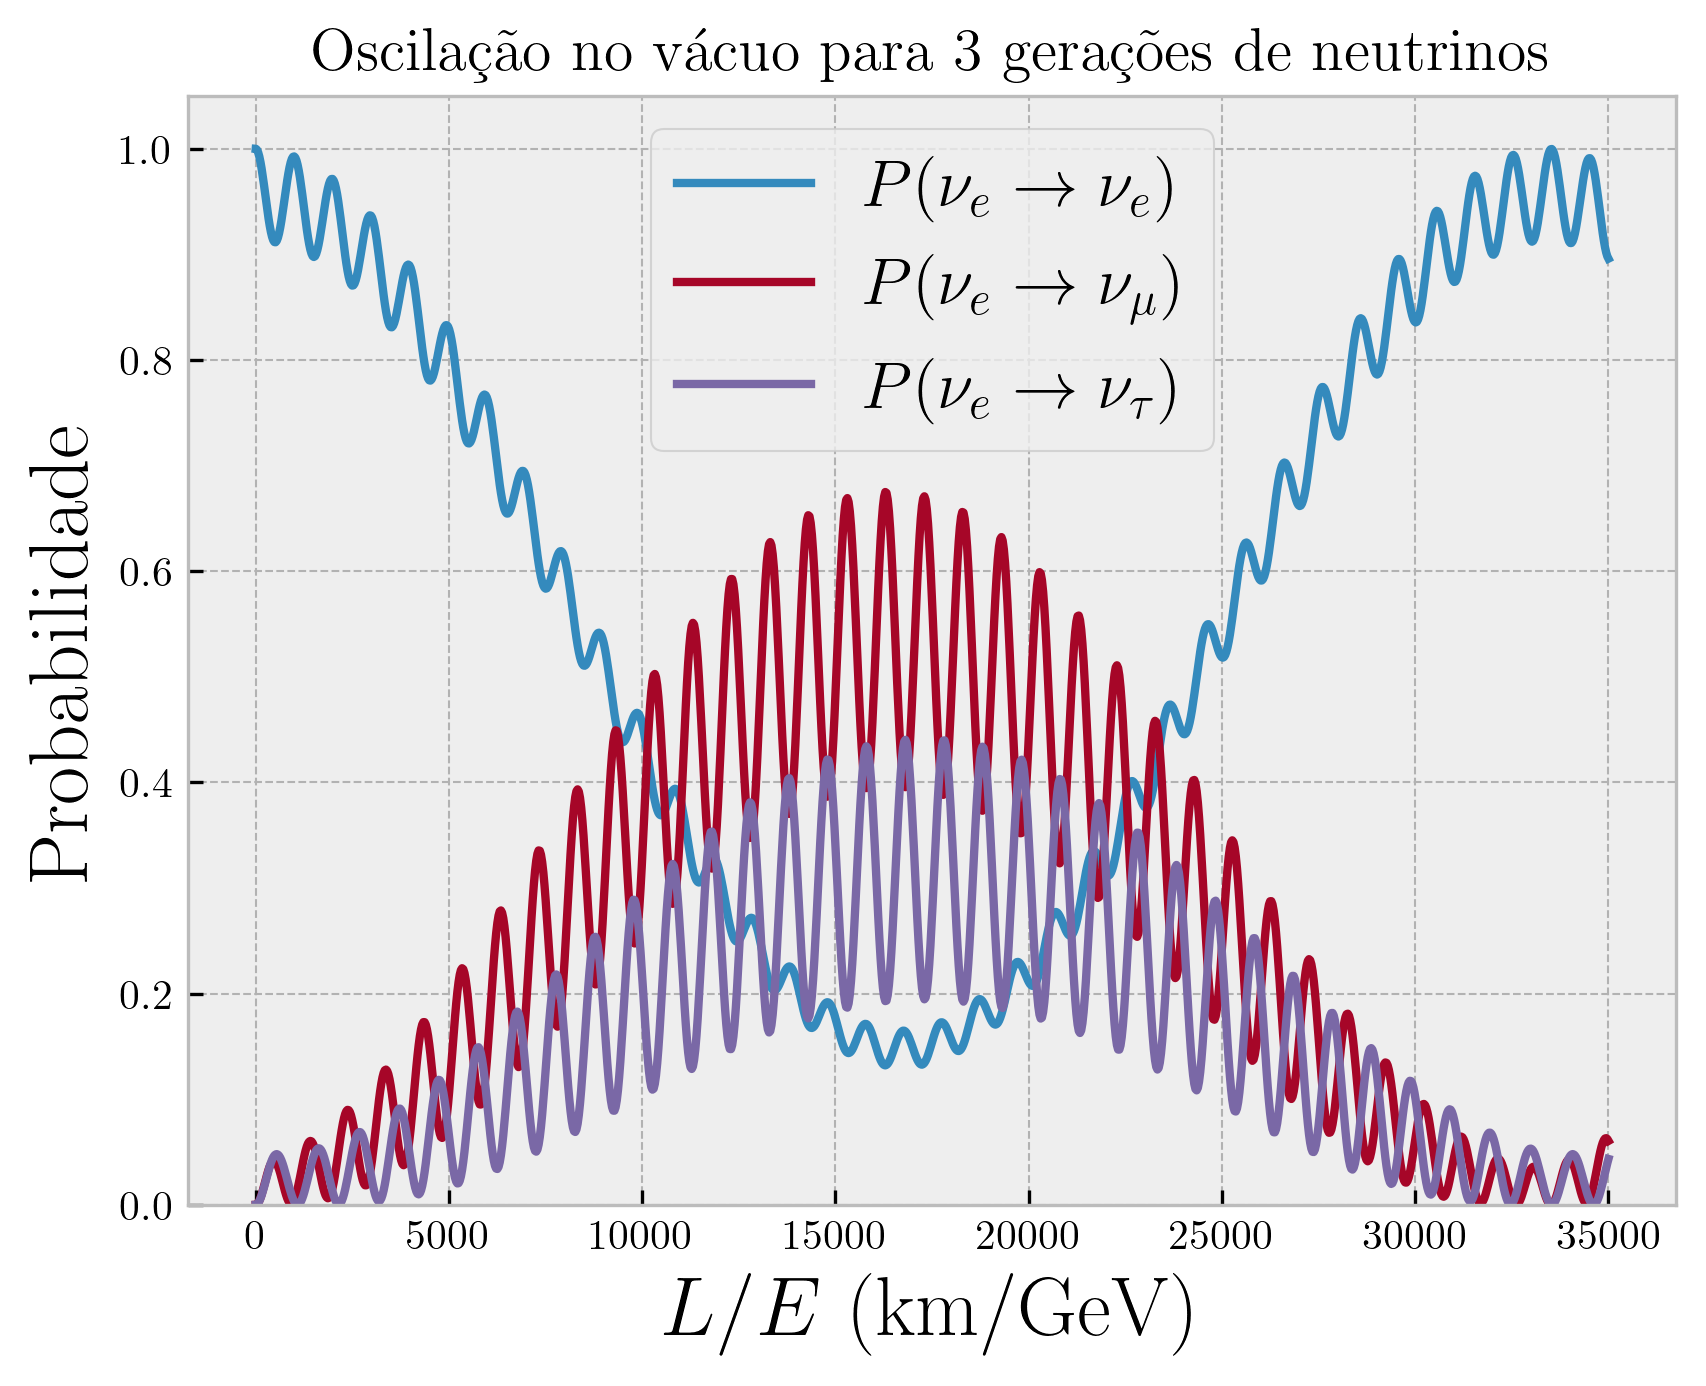
\includegraphics[width=.95\linewidth]{fig/3nu-vacuo-e.png}
  \caption{}
  \label{fig:vacuo-e}
\end{subfigure}%
\begin{subfigure}{.5\textwidth}
  \centering
  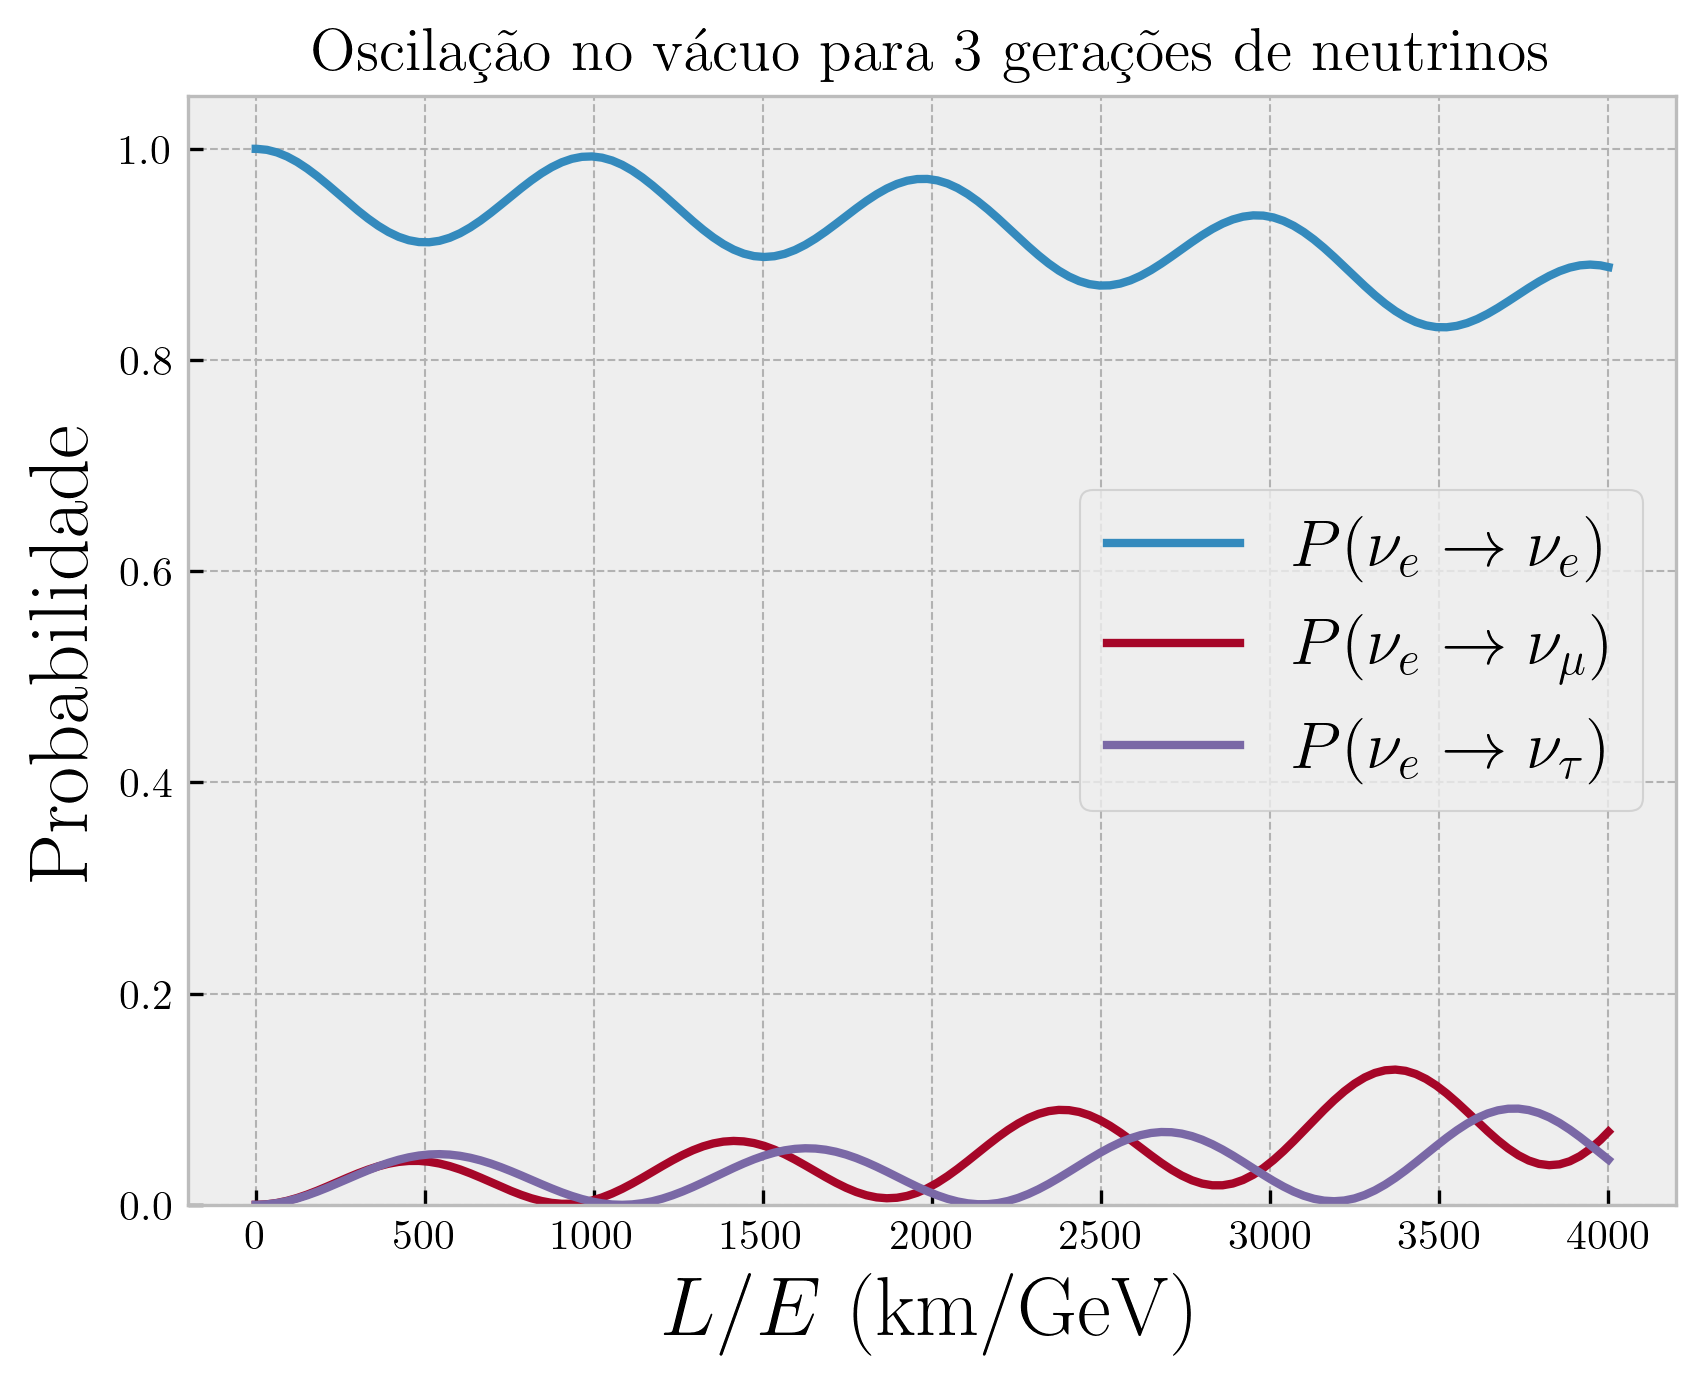
\includegraphics[width=.95\linewidth]{fig/3nu-vacuo-e_short.png}
  \caption{}
  \label{fig:vacuo-e_short}
\end{subfigure}
\caption{Probabilidades de transição de um neutrino no vácuo utilizando os parâmetros de melhor ajuste para NO dado pelo NuFIT \cite{nufit}, assumindo três gerações $\nu_e$, $\nu_\mu$ e $\nu_\tau$.}
\label{fig:vacuo_electron}
\end{figure}

\section{Neutrinos solares} \label{sec:solar-nu}

O Sol é uma estrela em que suas reações nucleares internas não possuem energia suficiente para produzir os léptons mais pesados $\mu^-$ e $\tau^-$. Dessa forma, todos os neutrinos emitidos pelo Sol são produzidos inicialmente em seu interior no estado de neutrino do elétron $\nu_e$.

Para uma geração de 3 neutrinos oscilando na matéria, a evolução é bem parecida com a equação \ref{eq:3nu-vacuo}. A única diferença é na hamiltoniana, que terá um potencial efetivo $V_e$ somente em sua componente $\ket{\nu_e}$, já que o neutrino $\nu_e$ do elétron é o único que interagirá com a densidade eletrônica no Sol.

A dedução da expressão $V_e = \sqrt{2} \, G_F N_e \, \text{diag}(1,0,0)$ pode ser encontrada em \cite{gonzalez}, onde $N_e(L)$ é a densidade eletrônica no interior do Sol e $G_F$ é a constante de Fermi da interação fraca. Com isso, a equação de evolução se escreve
\begin{equation} \label{eq:evol}
i \dv{t}
\begin{pmatrix}
\psi_e \\ \psi_\mu \\ \psi_\tau
\end{pmatrix}
= \qty[ \frac{1}{2E} \; U
\begin{pmatrix}
0 & 0 & 0 \\
0 & \Delta m_{21}^2 & 0 \\
0 & 0 & \Delta m_{31}^2 \\
\end{pmatrix}
U^\dagger +
\begin{pmatrix}
\sqrt{2} \, G_F N_e(t) & 0 & 0 \\
0 & 0 & 0 \\
0 & 0 & 0 \\
\end{pmatrix}
]
\begin{pmatrix}
\psi_e \\ \psi_\mu \\ \psi_\tau
\end{pmatrix},
\end{equation}
onde $U$ é dada pela equação \ref{eq:mixmatrix}.


\subsection{Abordagem numérica} \label{sec:magnus}

O problema de interesse é resolver uma equação de Schrödinger
\begin{equation} \label{eq:schrodinger}
i \dv{\Psi}{t} = H \Psi,
\end{equation}
para qual implementamos o algoritmo denominado ``expansão de Magnus'' \cite{efficient-nu}. Este algoritmo consiste na representação exponencial (série de Dyson) da solução da equação de Schrödinger \ref{eq:schrodinger}
\begin{equation} \label{eq:omega}
\Psi(t) = e^{-i \Omega(t, t_0)} \Psi_0,
\end{equation}
onde $\Omega(t, t_0) =  \sum_{k=1}^{\infty} \Omega_k(t, t_0)$ e cada $\Omega_k$ é dado por múltiplas integrais envolvendo comutadores de $H(t)$.

A ideia do algoritmo então consiste em aplicar iterações
\begin{equation} \label{eq:omega-it}
\Psi(t_{n+1} = t_{n} + h_n) = e^{-i \Omega^{(p)}(t_n + h_n, t_n)} \Psi(t_n),
\end{equation}
onde truncamos $\Omega^{(p)} = \sum_{k=1}^{p} \Omega_k(t_n + h_n, t_n)$ em $p = m-2$, sendo $m + 1$ a ordem do erro de $\Psi(t_n)$ em cada iteração.

Em nosso caso utilizamos a expansão de Magnus em ordem 4 (M4), onde $p = 2$. Seguindo \cite{efficient-nu}, aproximamos $\Omega^{(2)}$ através da quadratura de Gauss-Legendre de 2 pontos. Assim, definindo para cada iteração $\xi_{\pm} = t_n + \qty(1 \pm \frac{1}{\sqrt{3}}) \frac{h_n}{2}$ e $H_{\pm} = H(\xi_{\pm})$, temos que
\begin{equation} \label{eq:quadrature}
\Omega^{(2)}(t_n + h_n, h_n) = (H_+ + H_-) \frac{h_n}{2} +
i \frac{\sqrt{3}}{12} [H_-, H_+] h_n^2.
\end{equation}

A partir da equação \ref{eq:quadrature}, apenas nos resta calcular a exponencial de matriz \ref{eq:omega-it}. Fizemos esse cálculo através da diagonalização $\Omega = U^\dagger D U$, onde $D$ é uma matriz diagonal real e $U$ é unitária, portanto $e^{-i \Omega} = U^\dagger e^{-i D} U$.

\subsection{Resultados} \label{sec:solar-results}

Realizamos todos os cálculos envolvendo neutrinos solares em linguagem \texttt{C} com o auxílio da biblioteca GNU Scientific Library (GSL) \cite{gsl}.

Consideramos os neutrinos produzidos pelas principais reações internas do Sol pelo modelo solar \texttt{BS2005} \cite{bahcall-model}. A Figura \ref{fig:raio} apresenta o gráfico das densidades de probabilidade $p$ de um neutrino de uma reação específica ser produzido no raio $R = r \, R_{\odot}$ dentro do Sol, sendo $R_\odot = 6.957 \times 10^8 \unit{m}$ o raio solar.

Através da interpolação da densidade eletrônica no interior do Sol, obtemos a função $N_e(t)$ a partir dos dados do modelo solar \href{http://www.sns.ias.edu/~jnb/SNdata/sndata.html#bs2005}{\texttt{BS2005}} \cite{bahcall} do website de John N. Bahcall. Pela implementação do algoritmo M4, calculamos a probabilidade de sobrevivência $P_{\nu_e \to \nu_e}(R)$ ao sair do Sol dado que $\nu_e$ foi produzido em seu interior no raio $R$. Assim, tomamos a média no ponto de produção
\begin{equation} \label{eq:media-raio}
\ev{P(\nu_e \to \nu_e)} = \int_0^{R_\odot} p(R) P_{\nu_e \to \nu_e}(R) \dd{R},
\end{equation}
o que nos possibilitou obter a Figura \ref{fig:surv_prob}, que exibe $\ev{P(\nu_e \to \nu_e)}$ para cada reação em função da energia $E$.

\begin{figure}[H]
\centering
\begin{subfigure}{.5\textwidth}
  \centering
  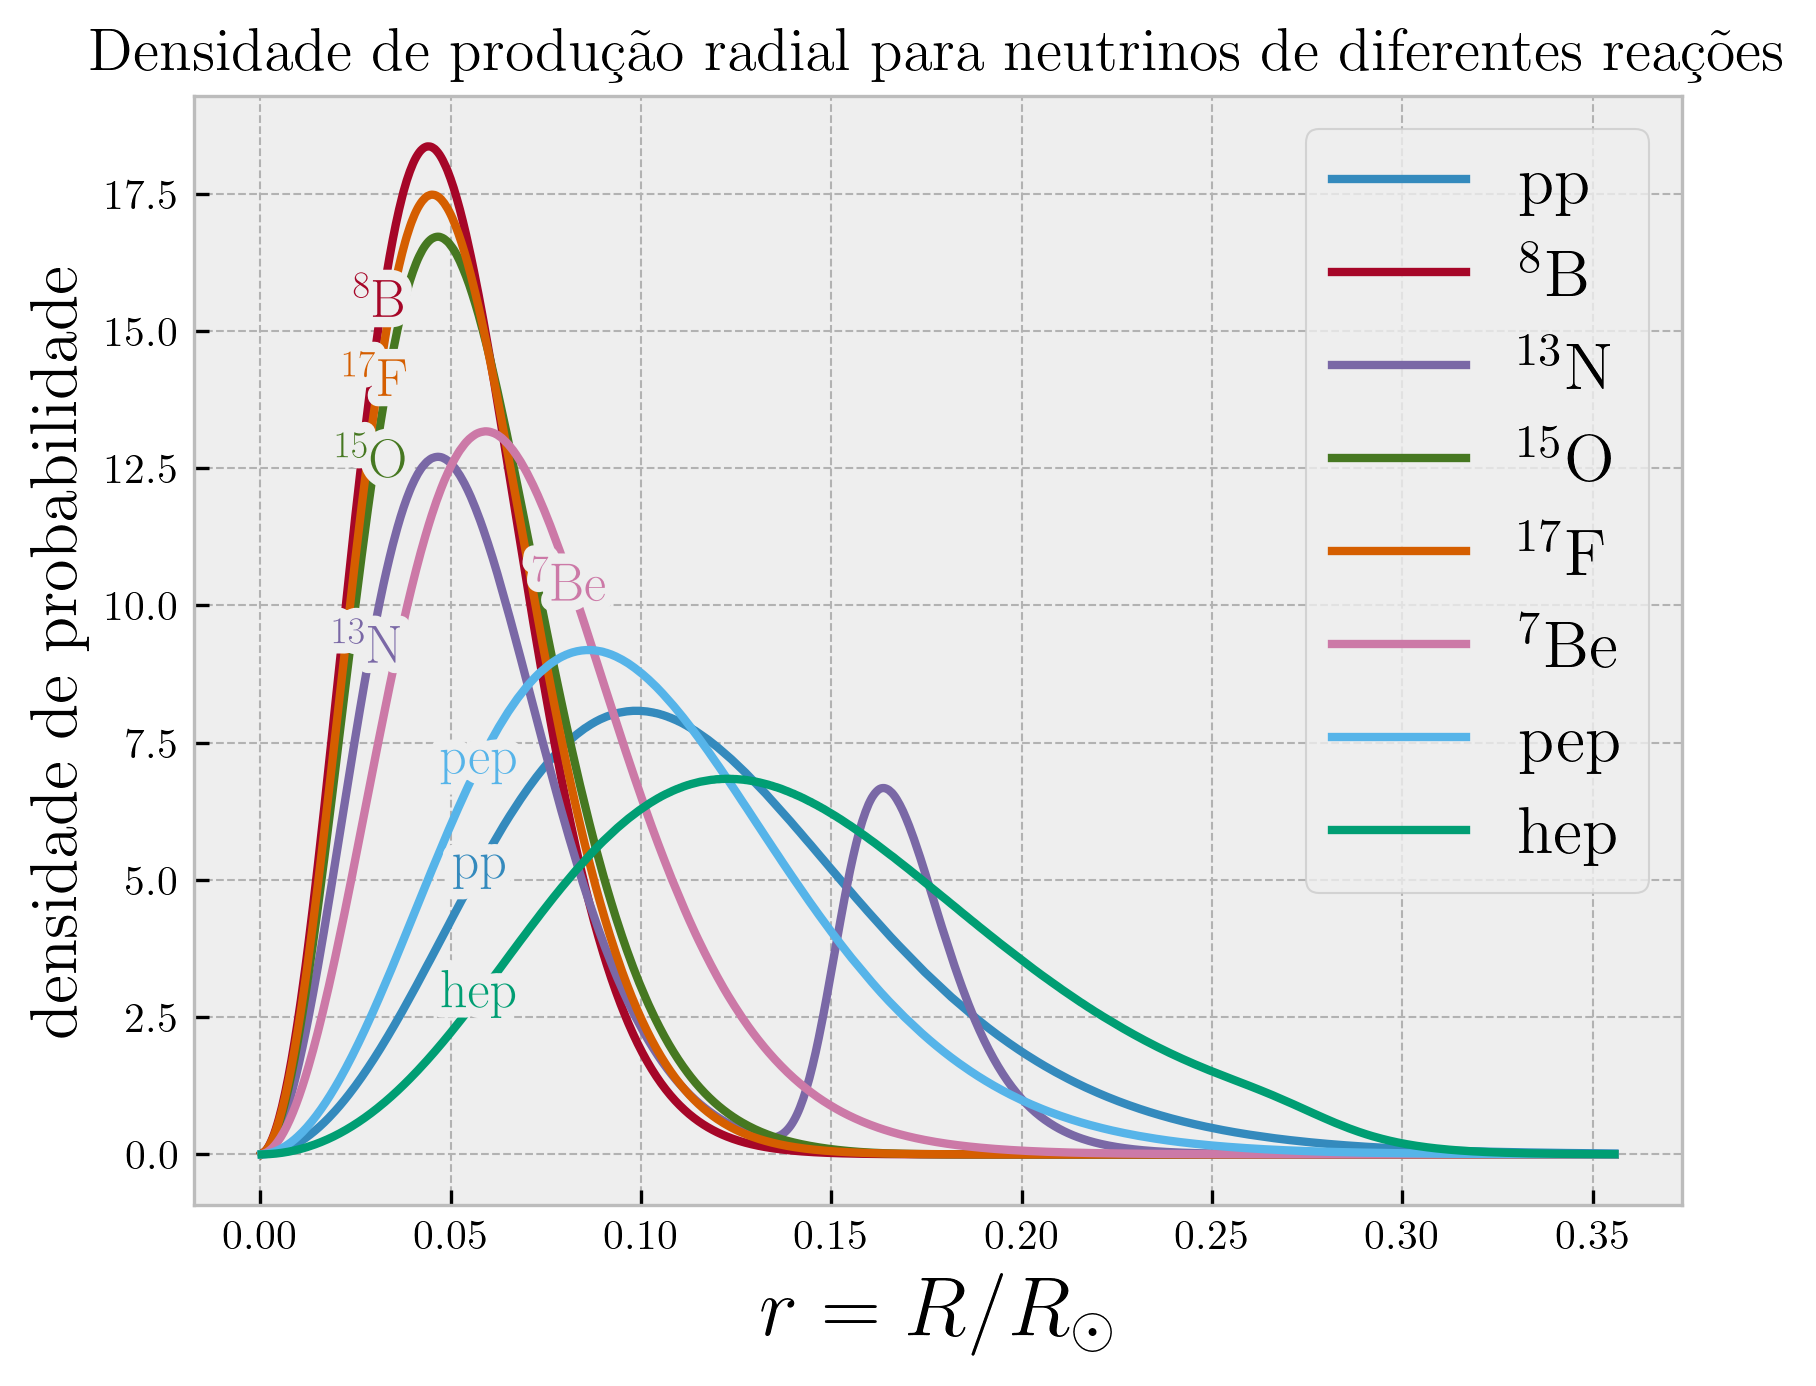
\includegraphics[width=\linewidth]{fig/raio.png}
  \caption{}
  \label{fig:raio}
\end{subfigure}%
\begin{subfigure}{.5\textwidth}
  \centering
  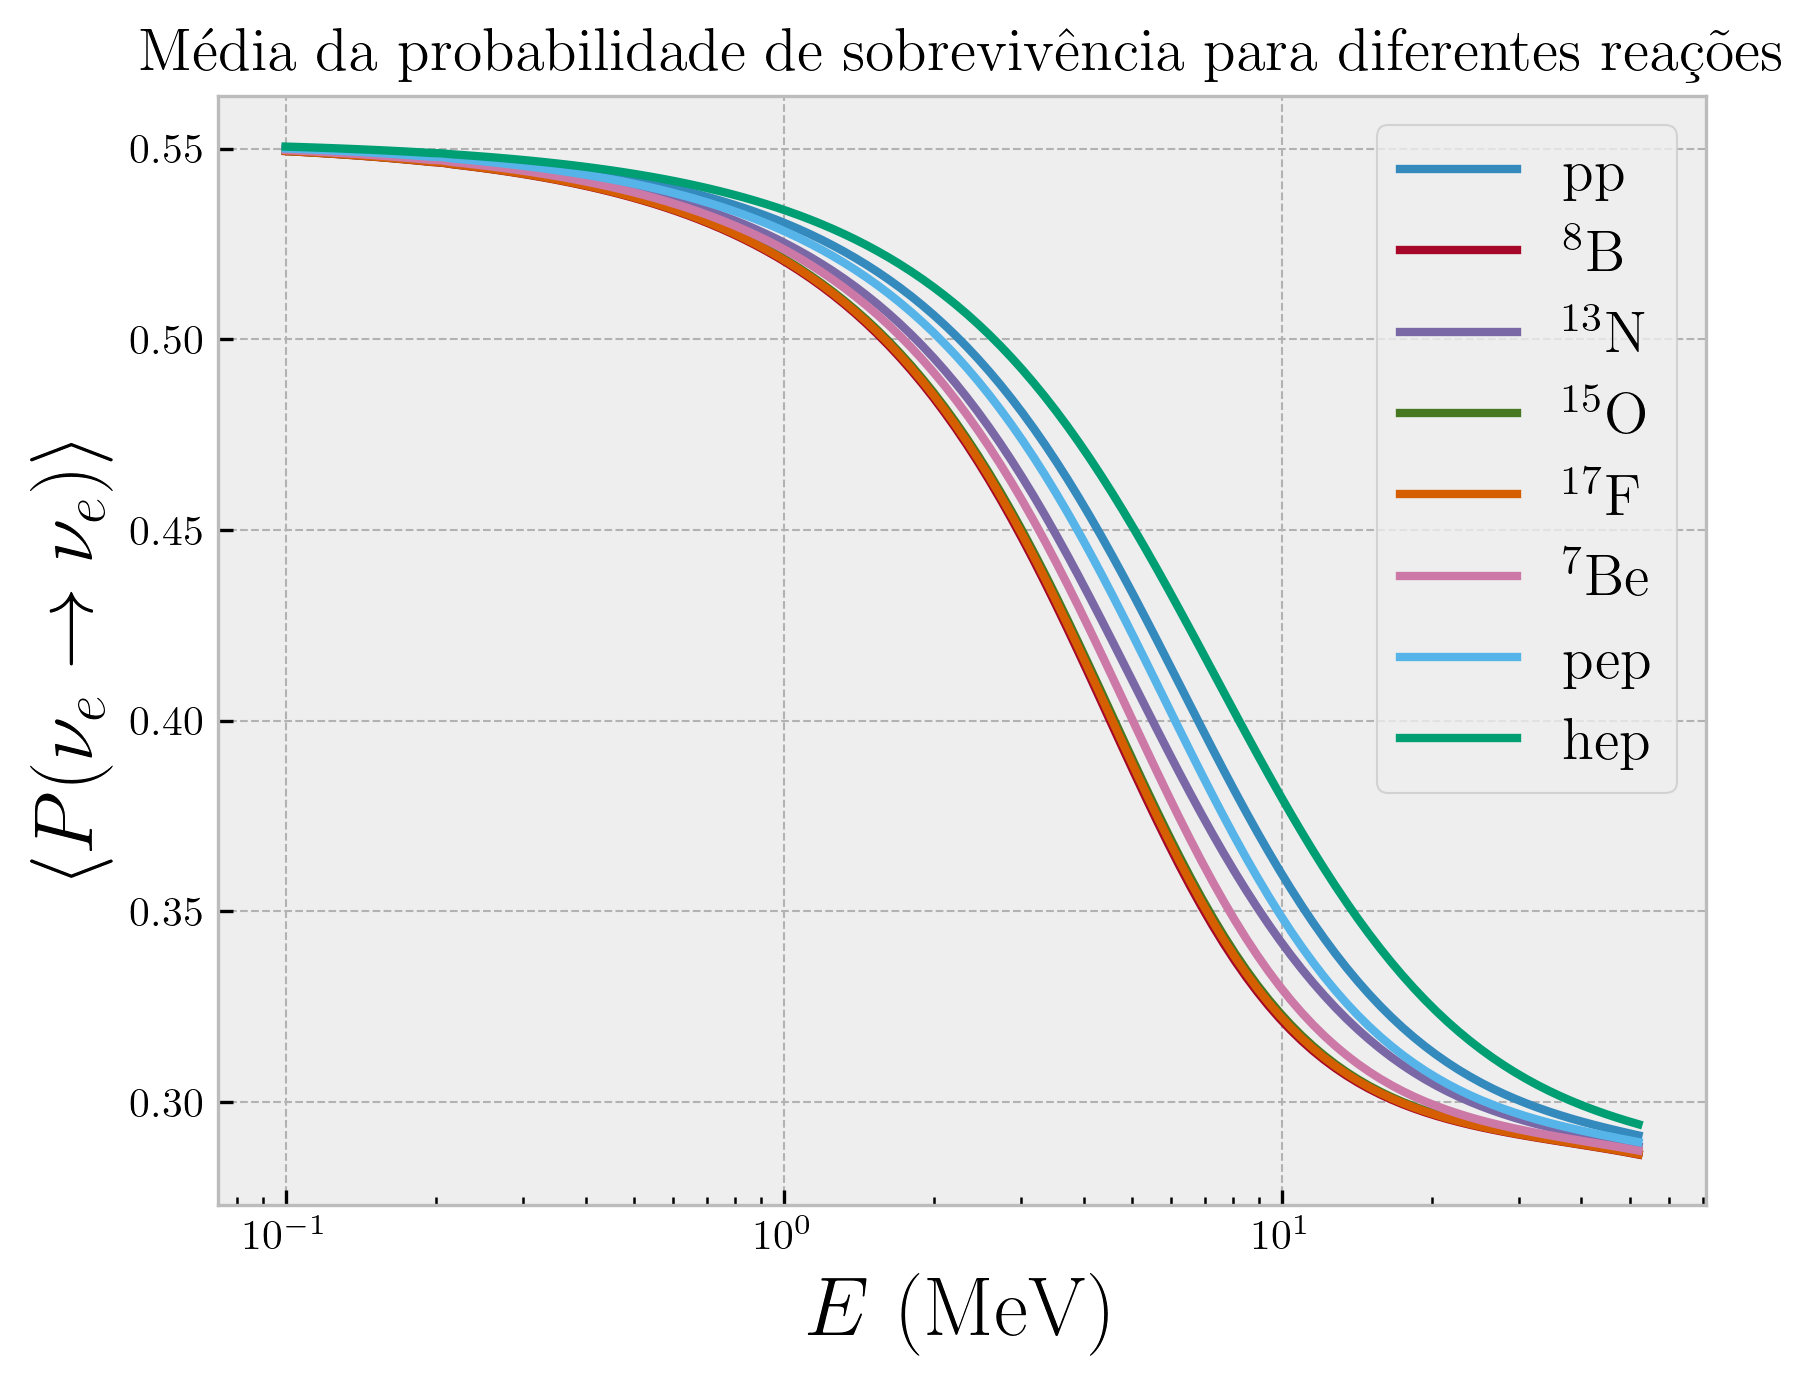
\includegraphics[width=\linewidth]{fig/surv_prob.png}
  \caption{}
  \label{fig:surv_prob}
\end{subfigure}
\caption{Densidades de produção radial de neutrinos e suas respectivas probabilidades médias de sobrevivência $\ev{P(\nu_e \to \nu_e)}$ ao sair do Sol como função da energia $E$.}
\label{fig:solar_results}
\end{figure}


\section{KamLAND} \label{sec:kamland}

O KamLAND é um experimento que detecta antineutrinos $\cc{\nu}_e$ produzidos principalmente por reatores nucleares. Os antineutrinos são detectados pelo decaimento $\beta$ inverso
\begin{equation} \label{eq:inverse-beta}
\cc{\nu}_e + p \to e^+ + n,
\end{equation}
em que são contabilizados todos os eventos detectados em função da energia do pósitron $E_{e^+} = E - \Delta M$, onde $E$ é a energia do antineutrino e $\Delta M = m_n - m_p - m_e = 0.782 \unit{MeV}$. Sendo feita a contagem, o resultado é comparado com a distribuição de eventos esperada, que é calculada supondo que a maior parte dos antineutrinos detectados foram produzidos pelos reatores nucleares ao redor do KamLAND.

\subsection{Simulação numérica} \label{sec:kamland-simul}

Realizamos uma simulação do KamLAND no período correspondente ao artigo \cite{spectral-distortion} de 9 de Março, 2002 a 11 de Janeiro, 2004. Obtemos a distribuição de eventos esperada e a comparamos com os dados disponibilizados \cite{kamland-data}. Para calcular a distribuição de eventos, consideramos as mesmas usinas nucleares do artigo \cite{stanford-reactors}, que incluem 52 reatores no Japão e 18 reatores na Coréia do Sul. Para realizar essa simulação, são necessárias apenas quatro informações \cite{refmodel} para cada reator $k$:
\begin{enumerate}
\item o tipo do reator: PWR, BWR, GCR, LWGR, MOX ou PHWR \cite{refmodel}.
\item a distância $d_k$ ao experimento KamLAND.
\item a potência térmica $P_{\text{th}}^k$ do reator.
\item o \textit{average load factor} $L_F^k$ do período considerado, que corresponde à fração da operação efetiva com respeito ao seu funcionamento ideal.
\end{enumerate}

Todas essas informações estão disponíveis na base de dados PRIS \cite{pris-iaea} da International Atomic Energy Agency (IAEA). A Tabela \ref{table:reactors} mostra os parâmetros numéricos para todas as usinas nucleares consideradas, enquanto que a Figura \ref{fig:kamland-map} mostra um mapa com a localização dos reatores ao redor do KamLAND.

\begin{table}[ht]
\begin{minipage}[b]{0.49\linewidth}
\centering
\resizebox{\textwidth}{!}{ %
\begin{tabular}{ | c | c | c | c |}
\hline
\textbf{Japão}         & Distância & $P_{\text{th}}$ (GW) & $L_F$ $(\%)$ \\ \hline
Kashiwazaki (7)        & 160 km    & 24.317 &  52.9             \\ \hline
Ohi (4)                & 179 km    & 13.692 &  90.2             \\ \hline
Takahama (4)           & 191 km    & 10.200 &  89.2             \\ \hline
Tsuruga (2)            & 138 km    & 4.481  &  86.7             \\ \hline
Hamaoka (4)            & 214 km    & 10.615 &  41.2             \\ \hline
Mihama (3)             & 146 km    & 4.927  &  85.1             \\ \hline
Shika (1)              & 88  km    & 1.593  &  57.2             \\ \hline
Fukushima Daiichi (6)  & 349 km    & 14.197 &  51.1             \\ \hline
Fukushima Daini (4)    & 345 km    & 13.172 &  39.0             \\ \hline
Tokai-II (1)           & 295 km    & 3.293  &  84.3             \\ \hline
Onagawa (3)            & 431 km    & 6.465  &  72.8             \\ \hline
Shimane (2)            & 401 km    & 3.816  &  79.2             \\ \hline
Ikata (3)              & 561 km    & 5.960  &  84.2             \\ \hline
Genkai (4)             & 755 km    & 10.146 &  89.8             \\ \hline
Sendai (2)             & 830 km    & 5.320  &  85.0             \\ \hline
Tomari (2)             & 783 km    & 3.300  &  83.3             \\ \hline \hline
\textbf{Coréia do Sul} & Distância & $P_{\text{th}}$ (MW) & $L_F$ $(\%)$ \\ \hline
Hanul (4)              & 712 km    & 11.200 &  84.7             \\ \hline
Wolsong (4)            & 986 km    & 8.244  &  95.0             \\ \hline
Hanbit (6)             & 735 km    & 16.874 &  87.8             \\ \hline
Kori (4)               & 709 km    & 9.435  &  98.3             \\ \hline
\end{tabular}
}
\caption{Reatores nucleares no Japão e Coréia do Sul que estavam em funcionamento durante o período analisado \cite{pris-iaea}.}
\label{table:reactors}
\end{minipage}\hfill
\begin{minipage}[b]{0.47\linewidth}
    \centering
    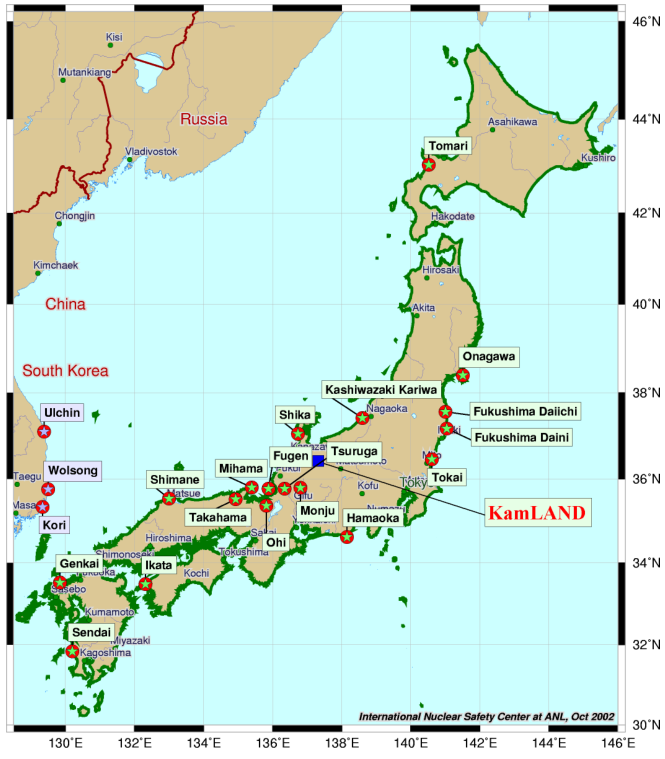
\includegraphics[width=\textwidth]{fig/kamland-map.png}
    \captionof{figure}{Localização dos reatores ao redor do experimento KamLAND. Figura retirada de \cite{detwiler}.}
    \label{fig:kamland-map}
    \end{minipage}
\end{table}

Na análise considerada \cite{spectral-distortion}, os eventos foram divididos em 13 sítios de energia igualmente espaçados por $0.425 \unit{MeV}$. O número de eventos em cada sítio $N_i$ é dado por \cite{juno}
\begin{equation} \label{eq:n_events}
N_i = N_{\s{T}} \int \dd{E}
\int_{E_i^{\text{min}}}^{E_i^{\text{max}}} \dd{E'}
\phi_{\cc{\nu}_e}(E) \sigma(E) R(E, E'),
\end{equation}
onde $N_{\s{T}} = n_p \s{E} \s{T}$ é uma constante de normalização que leva em conta o tempo de exposição $\s{T}$, a eficiência do detector $\s{E}$ e o número de prótons alvos $n_p$ para a reação \ref{eq:inverse-beta}; $\phi_{\cc{\nu}_e}(E)$ é o fluxo total de antineutrinos no KamLAND; $\sigma(E)$ é a seção de choque da reação \ref{eq:inverse-beta} e $R(E, E')$ é a função de resolução de energia do experimento.

A função $R(E, E')$ tem uma forma gaussiana \cite{juno}
\begin{equation} \label{eq:resol_func}
R(E, E') = \frac{1}{\sqrt{2\pi} \, \sigma_E(E)} \,
\exp(-\frac{(E-E')^2}{2 \sigma_E^2(E)}),
\end{equation}
onde $\sigma_E(E)$ é a resolução de energia. Os parâmetros utilizados para obter $N_{\s{T}}$ e $R(E, E')$ estão disponíveis na página \cite{kamland-data}, que acompanha a referência \cite{spectral-distortion}.

Para a seção de choque do decaimento $\beta$ inverso, utilizamos a aproximação \cite{cross-sec}
\begin{equation} \label{eq:cross-sec}
\sigma(E) = p_{e^+} E_{e^+}
E^{-0.07056 + 0.02018 \ln(E) - 0.001953 \ln^3(E)}
\times 10^{-43} \unit{cm^2}, \quad
p_{e^+} = \sqrt{E_{e^+}^2 - m_e^2}.
\end{equation}

O fluxo de antineutrinos é dado por \cite{refmodel}
\begin{equation} \label{eq:flux}
\phi_{\cc{\nu}_e}(E) =
\sum_{k}^{\text{reactors}} \frac{P_{\text{th}^k} L_F^k}{4 \pi d_k^2}
P_{\nu_e \to \nu_e}(E, d_k)
\sum_{i = 1}^{4} \frac{p_i^k}{Q_i} \lambda_i(E),
\end{equation}
onde são somadas as contribuições de todos os reatores ao redor do KamLAND e a probabilidade de sobrevivência $P_{\nu_e \to \nu_e}(E, d_k)$ é incluída assumindo invariância CPT (para calcularmos o fluxo supondo que não houvessem oscilações, basta colocarmos $P_{\nu_e \to \nu_e} \equiv 1$). O termo $\sum_{i = 1}^{4} \frac{p_i^k}{Q_i} \lambda_i(E)$ leva em conta os principais isótopos $^{235} \text{U}$, $^{238} \text{U}$, $^{239} \text{Pu}$ e $^{241} \text{Pu}$ responsáveis pela produção de antineutrinos através de fissões nucleares nos reatores. Os valores de $p_i^k$ e $Q_i$ estão disponíveis nas tabelas I e II de \cite{refmodel}. As funções $\lambda_i(E)$ foram obtidas através de um ajuste exponencial de um polinômio de ordem 5 para os espectros de energia dos antineutrinos de cada isótopo \cite{mueller}
\begin{equation} \label{eq:lambda}
\lambda_i(E) = \exp(\sum_{m=0}^{5} a_m^i E^m),
\end{equation}
onde os coeficientes $a_n^i$ estão disponíveis na Tabela VI de \cite{mueller}.

\subsection{Resultados} \label{sec:kamland-results}

A lista de eventos e o espectro de fundo do KamLAND correspondente ao período estão disponíveis em \cite{kamland-data}. Calculamos a distribuição de eventos sobre cada um dos 13 sítios pela equação \ref{eq:n_events} assumindo que não houvesse oscilação e assumindo que houvesse oscilação de duas gerações com os parâmetros $\Delta m_{21}^2 = 7.42 \cdot 10^{-5} \unit{eV^2}$ e $\theta_{12} = 33.44^\circ$ de outubro de 2021 do NuFIT \cite{nufit}. Para a simulação com oscilação adicionamos o espectro de fundo e utilizamos as incertezas descritas em \cite{spectral-distortion} para assim obter a Figura \ref{fig:kamland-events}.

\begin{figure}[H]
\centering
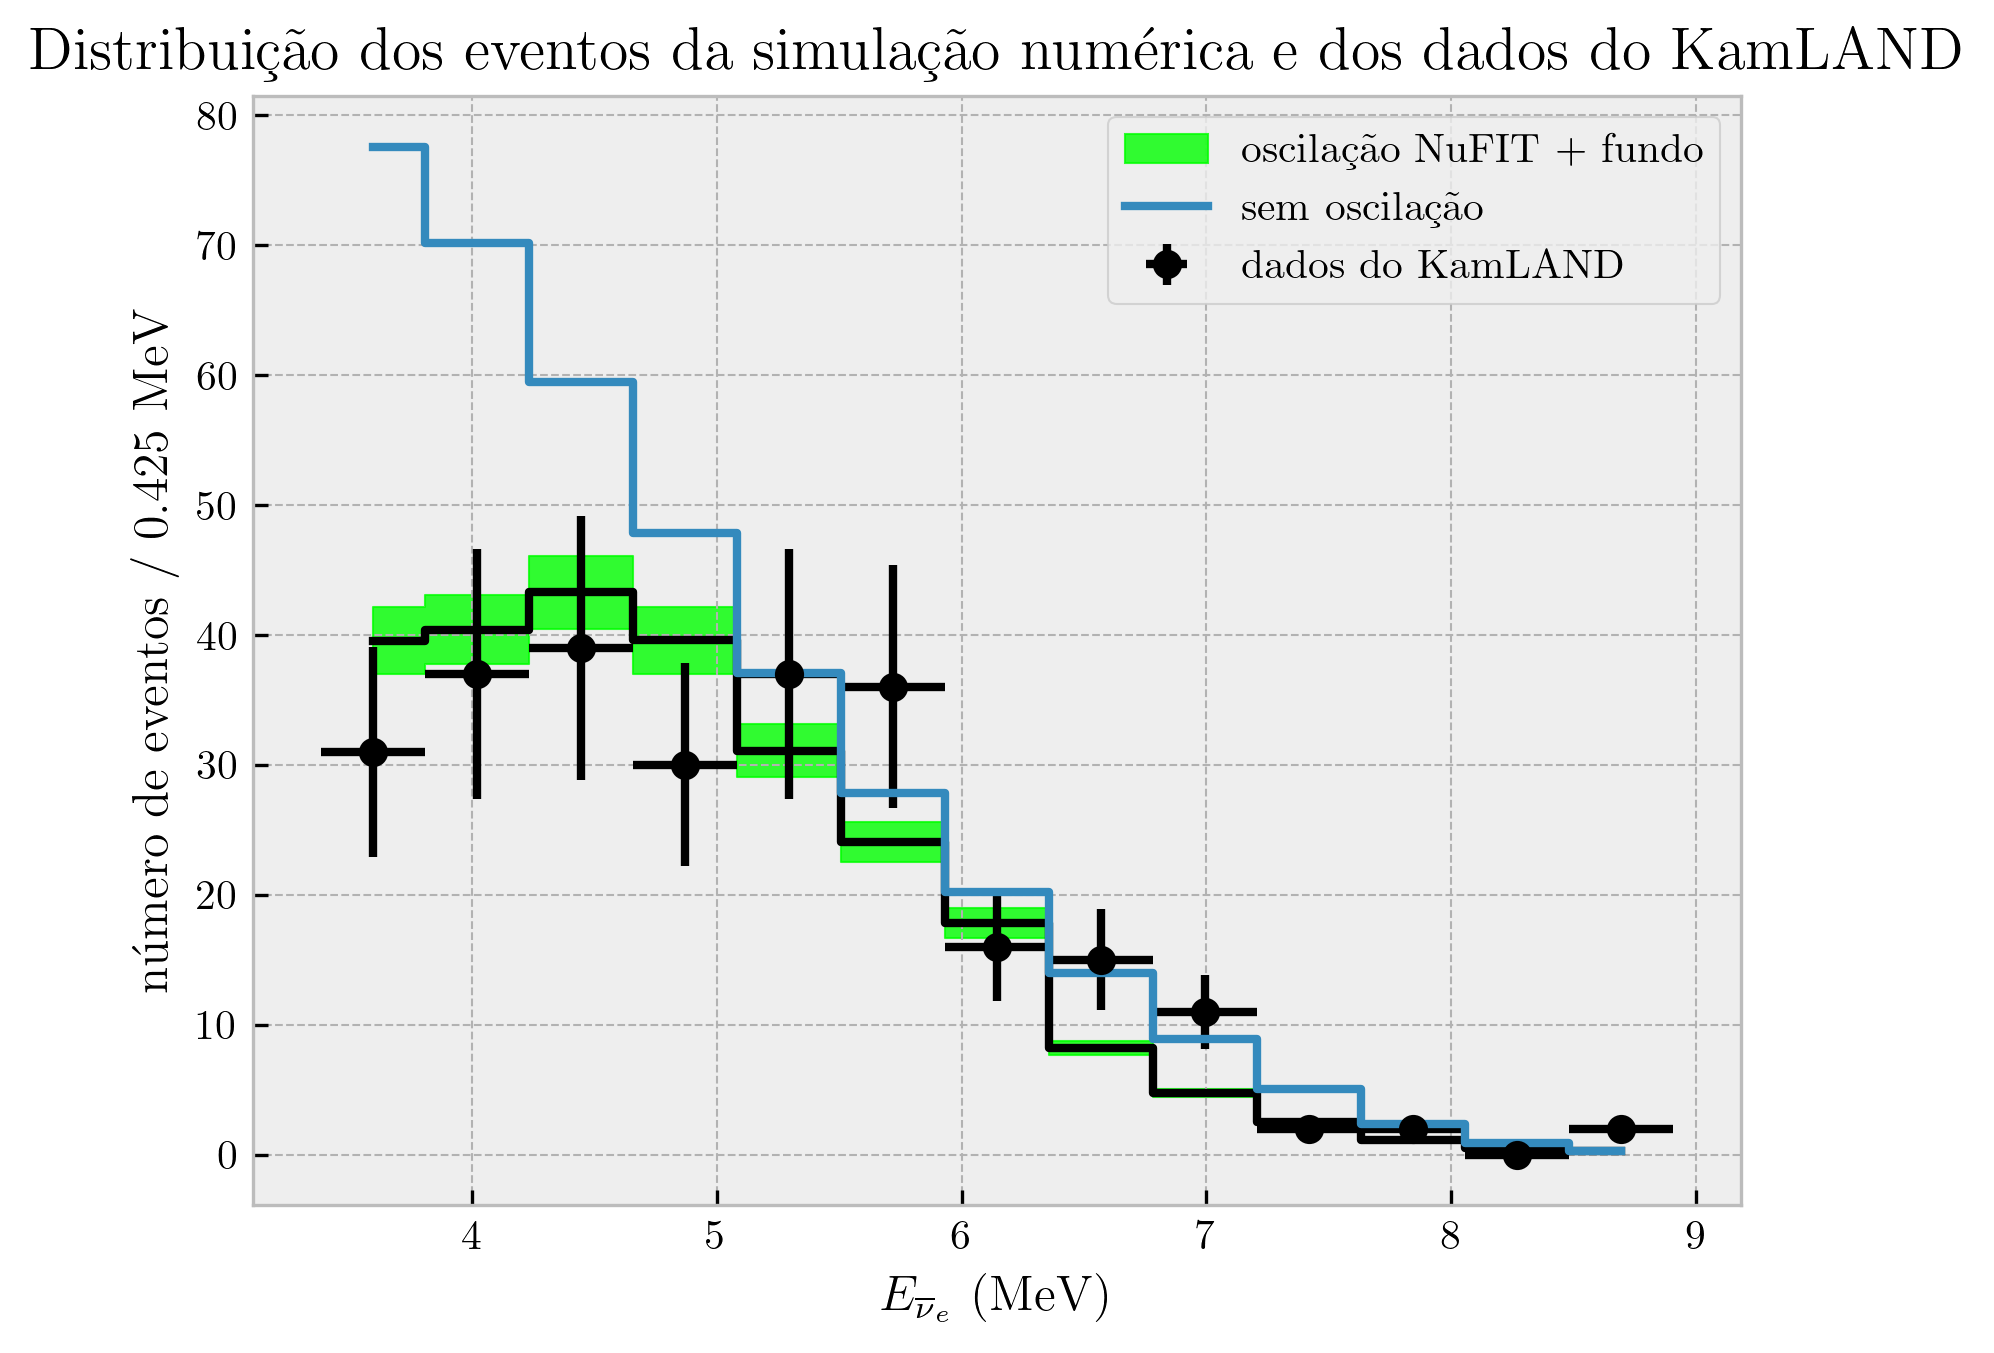
\includegraphics[width=0.85\textwidth]{fig/kamland-events.png}
\caption{Comparação entre a simulação numérica e os dados do KamLAND.}
\label{fig:kamland-events}
\end{figure}

Em nossa simulação, o número total de eventos sem oscilação foi $N_{\text{no-osc}} = 371.5 \pm 24.1$ enquanto que número total de eventos com oscilação para os valores dos parâmetros de melhor ajuste do NuFIT + (eventos de fundo) foi $N_{\text{osc}} = 253.1 \pm 16.5$.

Durante o período considerado, o experimento KamLAND detectou 258 eventos no total e a estimativa sem oscilação reportada em \cite{spectral-distortion} foi $365.2 \pm 23.7$ eventos.

\section{Conclusões}

Na seção \ref{sec:solar-nu} simulamos numericamente os neutrinos solares para diferentes reações. Os resultados obtidos na Figura \ref{fig:surv_prob} para a média no ponto de produção da probabilidade de sobrevivência ao sair do Sol estão de acordo com \cite{winslow}. Foi importante a implementação do algoritmo M4 \cite{efficient-nu}, que acelerou a execução do código na ordem de $10^3$ vezes.


Na seção \ref{sec:kamland} simulamos os eventos detectados pelo experimento KamLAND e obtivemos a Figura \ref{fig:kamland-events}, que está qualitativamente de acordo com os resultados de \cite{spectral-distortion}. Ainda mais, os resultados obtidos para o número total de eventos $N_{\text{no-osc}} = 371.5 \pm 24.1$ e $N_{\text{osc}} = 253.1 \pm 16.5$ são estatisticamente compatíveis dentro de uma incerteza com os 258 eventos realmente detectados pelo KamLAND e com a estimativa de $365.2 \pm 23.7$ eventos sem oscilação \cite{spectral-distortion}. Isso nos leva a concluir que os parâmetros atuais do NuFIT \cite{nufit} são compatíveis com o ajuste do KamLAND no período coberto por \cite{spectral-distortion}.


\chapter{Descrição e avaliação do Apoio Institucional recebido no período}\label{chp:apoioInst}

Durante o período correspondente a este relatório, o estudante não fez uso da reserva técnica.

\chapter{Participação em eventos científicos}\label{chp:particEvento}

O estudante apresentou seu projeto de iniciação científica na $30^{\text{a}}$ edição do \href{https://siicusp.prp.usp.br/pt/home/}{SIICUSP} e também participou de três workshops todos promovidos pelo \href{https://www.ictp-saifr.org/}{ICTP-SAIFR}:
\begin{itemize}
\item \href{http://journeys.ictp-saifr.org/}{V Journeys into Theoretical Physics, 2022}.
\item \href{https://www.ictp-saifr.org/qc2022/}{School on Quantum Computation, 2022}.
\item \href{https://www.ictp-saifr.org/cmtm2022/}{II ICTP-SAIFR Condensed Matter Theory in the Metropolis, 2022}.
\end{itemize}

\chapter{Disciplinas cursadas no período}

Durante o período coberto por este relatório, o estudante concluiu sua graduação em Física Bacharelado, havendo cursado apenas duas disciplinas em seu último semestre: ``Filosofia da Física'' e ``Aprendizado de Máquina e Reconhecimento de Padrões''.

\pagebreak

%%-----
%% Referências bibliográficas
%%-----
\addcontentsline{toc}{chapter}{\bibname}
%\bibliographystyle{abntex2-num}
\bibliography{bibliografia}
\bibliographystyle{ieeetr}

%%-----
%% Fim do documento
%%-----
\end{document}
